\documentclass{beamer}

\usetheme{Singapore}
\usecolortheme{dove}
\usefonttheme{structurebold}
\usepackage{graphicx}
\usepackage{color}
\usepackage{xcolor}
\usepackage[british]{babel}
\usepackage[all]{xy}

\title[Plastic Soup recognition]{Detecting Plastic Soup automatically\\ \it \large Using pre-trained Convolutional Neural Networks}
\subtitle[]{\normalsize Progress presentation}
\author[Y. Galama]{Student:\\Ysbrand Galama \\ 10262067 \\[2pc] Supervisor: Thomas Mensink\\}
\institute[UvA]
{
 
\includegraphics[width=0.7\textwidth]{images/uva-campus.pdf}
}
\date{29th May 2015}

\begin{document}

	\begin{frame}
	  \titlepage
	\end{frame}

\section{Introduction}
    \begin{frame}{Plastic Soup}
        \begin{itemize}
                \item Large amounts of plastic end up in the world ocean \cite{plastic}
                \item Automate the clean-up process
                \item Develop plastic soup recognition
        \end{itemize}
        \begin{columns}[c]
            \begin{column}{.5\textwidth}
            \end{column}
            \begin{column}{.5\textwidth}
                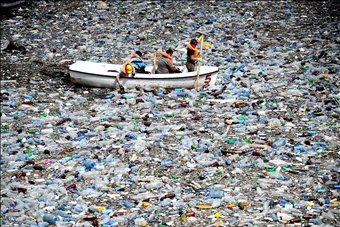
\includegraphics[width=\textwidth]{images/boat_in_plastic.jpg}\\{\small Figure 1: Boat in plastic soup}
            \end{column}
        \end{columns}
    \end{frame}
    
    \begin{frame}{Current state of the art image techniques}
        \begin{block}{Convolutional Neural Networks}
            \begin{itemize}
            \item Alexnet implementation to train large amounts of data \cite{alexnet}
            \item Current CNNs very high accuracy \cite{cnn}
            \end{itemize}
        \end{block}
        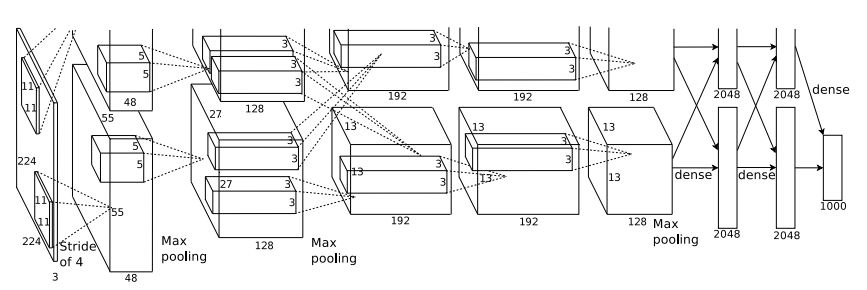
\includegraphics[width=\textwidth]{images/alexnet2012.png}
    \end{frame}
    \begin{frame}{Research question}
        \begin{block}{How does a pre-trained CNN perform when used for other classifications without being trained on a large amount of domain-specific data?}
        \end{block}
    \end{frame}
\section{Method}
    \begin{frame}{Dataset}
        \begin{columns}[c]
            \begin{column}{.5\textwidth}
                \begin{itemize}
                \item 37165 images from short films
                \item annotated by my hand
                \item 16553 images above and 20612 images below water
                \item 20635 show plastic only
                \item 6972 show animals only
                \item 8502 show both
                \end{itemize}
            \end{column}
            \begin{column}{.4\textwidth}
                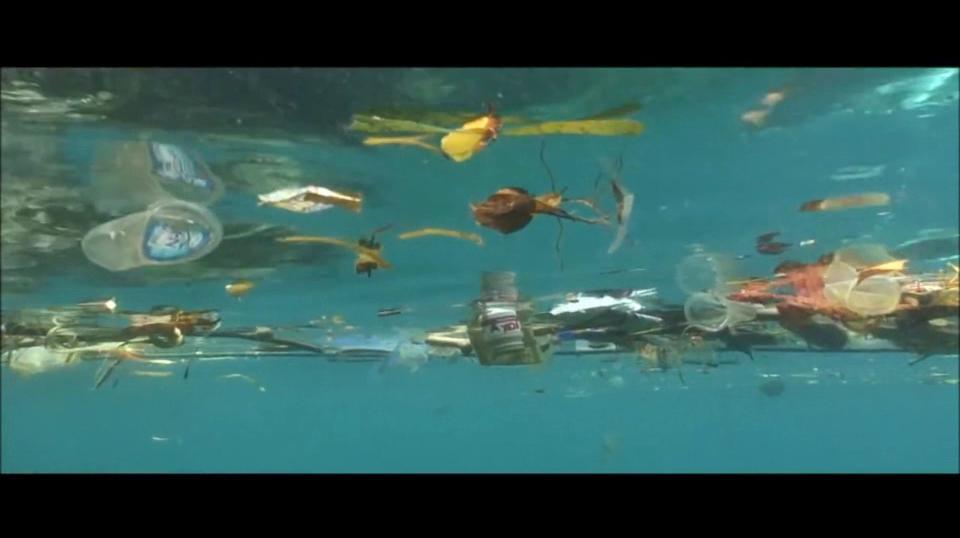
\includegraphics[width=\textwidth]{images/10947_01.jpg}\\
                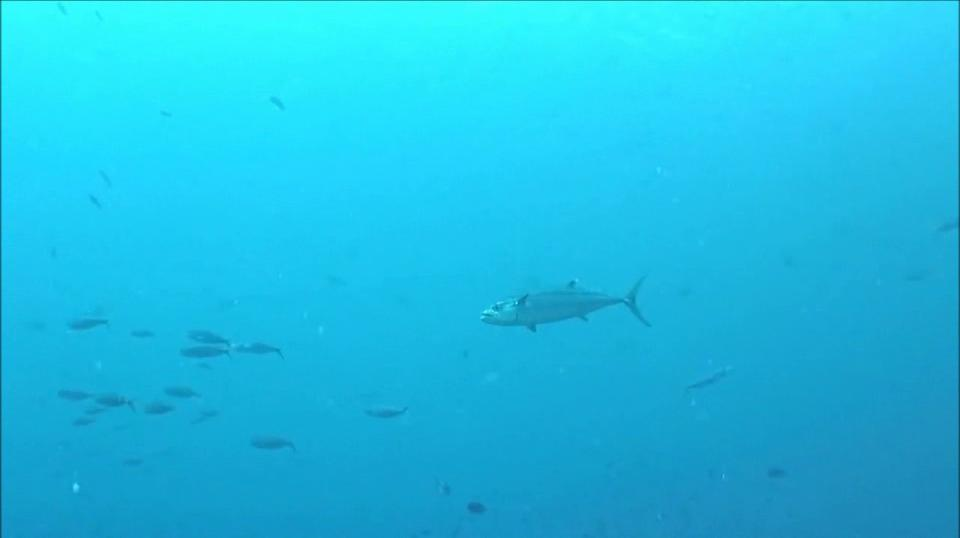
\includegraphics[width=\textwidth]{images/19358_10.jpg}\\
                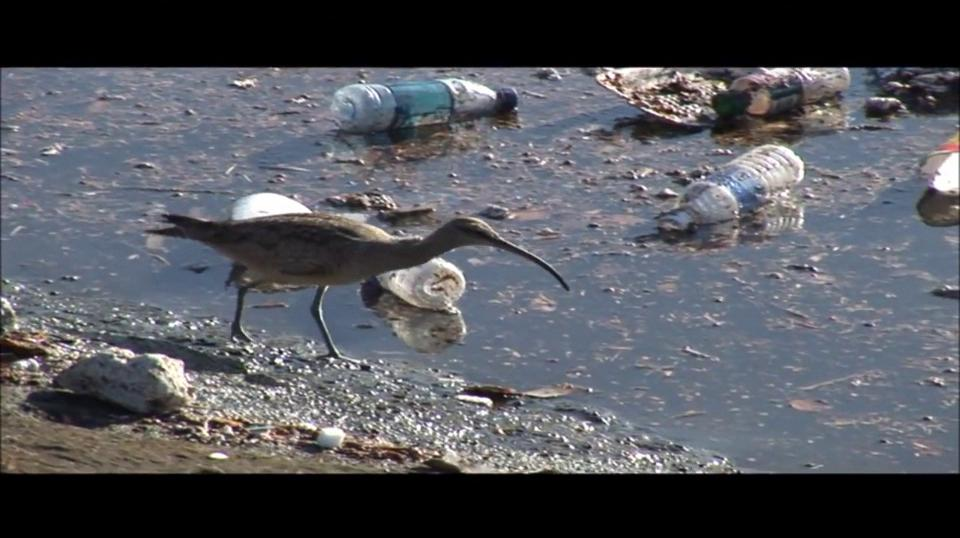
\includegraphics[width=\textwidth]{images/9077_11.jpg}\\
            \end{column}
        \end{columns}
    \end{frame}
    
    \begin{frame}{Method and evaluation}
        \begin{block}{Approach}
            \begin{itemize}
            \item Usage of a pre-trained Convolutional Neural Network
            \item Retrain the second-to-last layer for this specific domain
            \end{itemize}
        \end{block}
        \begin{block}{Evaluation}
            \begin{itemize}
            \item split dataset in train, validate and test
            \item score the results on the annotated data
            \end{itemize}
        \end{block}
    \end{frame}
\section{Results}
    \begin{frame}{Neural Network}
    \begin{block}{Approach}
        Using the train-set to train a single-hidden-layer neural network from the output of the CNN
    \end{block}
    \begin{block}{Results}
        \begin{itemize}
        \pause
        \item unsatisfactory results
        \item network did not learn
        \end{itemize}
    \end{block}
    \end{frame}
    
    \begin{frame}{Support Vector Machine}
    \begin{block}{Approach}
        Using the train-set to train a SVM, with the validate-set to investigate the parameters
    \end{block}
    \begin{block}{Results}
        \begin{itemize}
        \pause
        \item linear SVM model works best
        \item $99.9\%$ accuracy on the test-set
        \item $88.7\%$ accuracy on recognising plastic in other dataset
        \end{itemize}
    \end{block}
    \end{frame}
\section{Plan}
    \begin{frame}{Plan}
        \small
        \xymatrix @=.2pc @C=2pc @R=.2pc{
        \text{\bf old plan} & \text{\bf current plan} \\
        {\begin{array}{l}
            \text{Collect and annotate data} \\
            \text{Install CNN framework}
        \end{array}} \ar[d] & \\
        {\begin{array}{c}
            \text{Classify last layer of CNN}\\
            \text{(2 weeks)}
        \end{array}} 
        \ar[d] \ar[r]
        & \text{Classification took 3 weeks} \ar[d]\\
        {\begin{array}{c}
            \text{Find plastic within image} \\
            \text{(4 weeks)}
        \end{array}}
        \ar[d] & 
        {\begin{array}{c}
            \text{Writing first version of report} \\
            \text{(1 week)} \\
            \text{Improve current classifier} \\
            \text{(2 weeks)}
        \end{array}}\ar[d] \\
        {\begin{array}{c}
            \text{Write report} \\
            \text{(2 weeks)}
        \end{array}} &
        {\begin{array}{c}
            \text{Write final version of report} \\
            \text{(1 week)} \\
            \text{Finalise project} \\
            \text{(1 week)}
        \end{array}}
        }
    \end{frame}

    \begin{frame}[allowframebreaks]{References}
        \bibliographystyle{abbrv}
        \bibliography{Tex_sources/beamerbib}
    \end{frame}
\end{document}